%Start
%required packages and reason
\documentclass[11pt]{article}
\usepackage[a4paper,margin=1in]{geometry}
\usepackage{mathtools} % required for sigma notation
\usepackage{graphicx} %required to load images
\usepackage{amsmath} %required for the matrices
\usepackage{upgreek} %required for Greek symbols
\usepackage{xfrac} %for differentiation symbol
\usepackage{float} %to set the figures exactly where we want,(\figure "[H]")
\usepackage{listings} %to get colorful code in latex
\usepackage{color} %to get a nice color scheme
\usepackage{pythonhighlight} %to make the the python codes nice

%initial headings
\title{EE2703 Assignment 8: The Digital Fourier Transform}
\author{Anvith Pabba [EE19B070]}
\date{25th May 2021}

%begin document
\begin{document}

\maketitle

\section{Abstract}
The main objectives of the Assignment are:
\begin{itemize}
    \item Learning about DFT (Discrete Fourier Transform) and how it can be implemented in Python using the fft and fftshift function in numpys fft module. ( \textit{numpy.fft.fft()} )
    \item Using the fft function to find the DFTs of variuos periodic functions
    \item Plotting and analysing the relevent graphs
\end{itemize}

\section{Introduction to DFT}
\subsection{Theory}
Suppose f[n] is a periodic sequence of samples, with a period N. i.e:
\begin{equation}
    f[n] = f[n+N]
\end{equation}
Then the DTFT of the sequence is also a periodic sequence F[k] with the same period N. So we have:
\begin{equation}
    F[k] = \sum_{n=0}^{N-1}f[n]e^{-2\pi \frac{nk}{N} j} = \sum_{n=0}^{N-1}f[n]W^{nk}
\end{equation}
\begin{equation}
    f[n] = \frac{1}{N} \sum_{n=0}^{N-1} F[k]W^{-nk}
\end{equation}
Where,
\begin{equation}
    W = e^{-2\pi\frac{j}{N}}
\end{equation}
The values F[k] are what remains of the Digital Spectrum $F(e^{j\theeta})$. We can consider them as the values of $F(e^{j\theeta})$ for $\theeta = 2\pi \frac{k}{N}$,  since the first N terms in the expression for $F(e^{j2\pi \frac{k}{N}})$ yield:
\begin{equation}
    F(e^{j2\pi \frac{k}{N}}) = \sum_{n=0}^{N-1}f[n]e^{-\frac{2\pi kn}{N}j} + ...
\end{equation}
Which is the same as the DFT expression. The remaining terms are just repetitions of the above sum and help build up the delta function that is needed to take us from a continuous transform to a discrete impulse.\\~\\
From the above, we realize that the DFT is nothing but  a sampled version of the DTFT, which is the digital version of the analog Fourier Transform.\\~\\
In this assignment, we explore how to obtain the DFT, and how to recover the
analog Fourier Transform for some known functions by the proper sampling of the function.




\subsection{Implementing DFT in Python}
There are two commands in Python, one to compute the forward fourier transform and the other to compute the inverse transform. They are:
\begin{itemize}
    \item \textit{numpy.fft.fft()}
    \item \textit{numpy.fft.ifft()}
\end{itemize}
When we import pylab, both functions are imported into the local namespace.



\section{Spectrum of sin(5t)}
given the signal is sin(5t) which is periodic, we find the spectrum.
\begin{equation}
    y = sin(5t)
\end{equation}
\begin{equation}
    y = \frac{e^{j(5t)} - e^{j(-5t)}}{2j}
\end{equation}
So, the spectrum is:
\begin{equation}
    Y(w) = \frac{1}{2j}[\delta (w-5) - \delta (w+5)]
\end{equation}
We observe peaks at w= 5 and w= -5 with peak magnitudes of 0.5 and the respective phases are $-\frac{\pi}{2}$ and $\frac{\pi}{2}$.

\subsection{The Plots}
\begin{figure}[H]
    \centering
    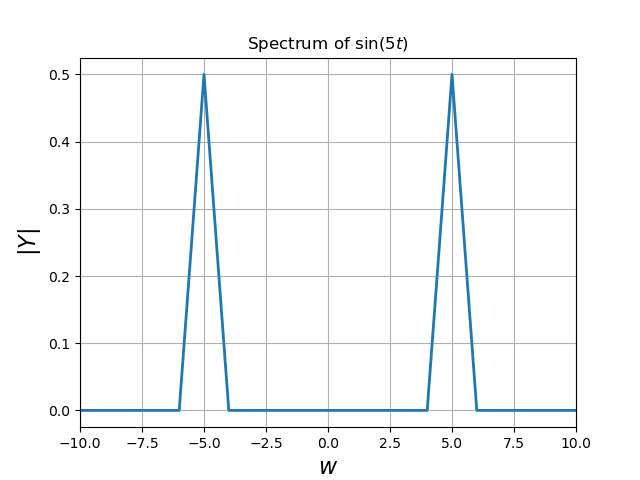
\includegraphics[scale = 0.75]{Figure_1a.png}
    \caption{Spectrum of sin(5t)}
\end{figure}
\begin{figure}[H]
    \centering
    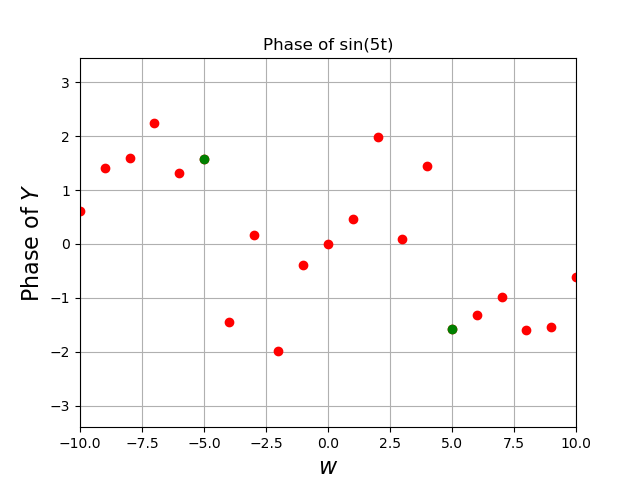
\includegraphics[scale = 0.75]{Figure_1b.png}
    \caption{Phase of sin(5t)}
\end{figure}

\subsection{The Code}
\begin{python}
#Q1: Working through the examples in the Assignment

#DFT of sin(5t)
x=linspace(0,2*pi,129);x=x[:-1]
y=sin(5*x)
Y=fftshift(fft(y))/128.0
w=linspace(-64,63,128)

#Magnitude plot of the DFT of sin(5t)
plot(w,abs(Y),lw=2)
xlim([-10,10])
ylabel(r"$|Y|$",size=16)
xlabel(r"$w$",size=16)
title(r"Spectrum of $\sin(5t)$")
grid(True)
show()

#Phase plot of the DFT of sin(5t)
plot(w,angle(Y),'ro',lw=2)
ii=where(abs(Y)>1e-3)				#plots the points in green only where magnitude is greater than 0.001
plot(w[ii],angle(Y[ii]),'go',lw=2)
xlim([-10,10])
ylabel(r"Phase of $Y$",size=16)
xlabel(r"$w$",size=16)
title('Phase of sin(5t)')
grid(True)
show()
\end{python}



\section{Spectrum of (1 + 0.1cos(t))cos(10t)}
\begin{equation}
    (1 + 0.1cos(t))cos(10t) = cos(10t) + 0.1(cos(t)*cos(10t))
\end{equation}
\begin{equation}
    cos(10t) + 0.1(cos(t)*cos(10t)) = cos(10t) + 0.05*cos(11t) + 0.05*cos(9t)
\end{equation}
\begin{equation}
\begin{array}{cc}
     cos(10t) + 0.05cos(11t) + 0.05cos(9t) &\\ = 0.5e^{j(10t)}+0.5e^{j(-10t)} +
     0.025e^{j(11t)}+0.025e^{j(-11t)} + 0.025e^{j(9t)}+0.025e^{j(-9t)}
\end{array}
\end{equation}
Hence,
\begin{equation}
    Y(w) = 0.5\delta (w-10) + 0.5\delta (w+10)+ 0.025\delta (w-11) + 0.025\delta (w+11)+ 0.025\delta (w-9) + 0.025\delta (w+9) 
\end{equation}
\\~\\
There fore, we have to have \textbf{6 peaks} in the spectrum

\subsection{With only 128 Samples}
Plots:
\begin{figure}[H]
    \centering
    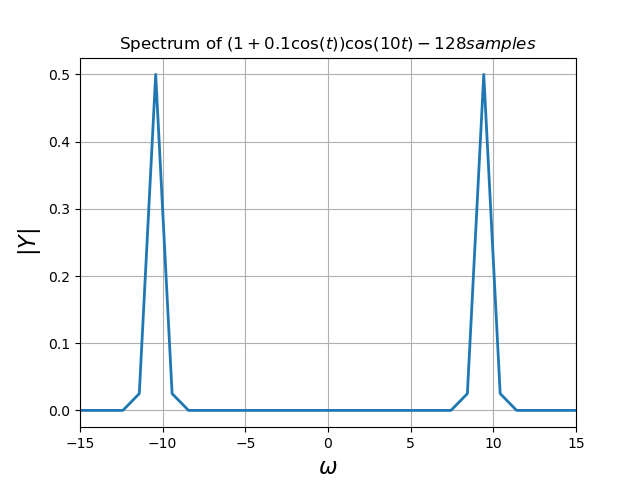
\includegraphics[scale = 0.75]{Figure_2a.png}
    \caption{Spectrum of (1 + 0.1cos(t))cos(10t) - 128 samples}
\end{figure}
\begin{figure}[H]
    \centering
    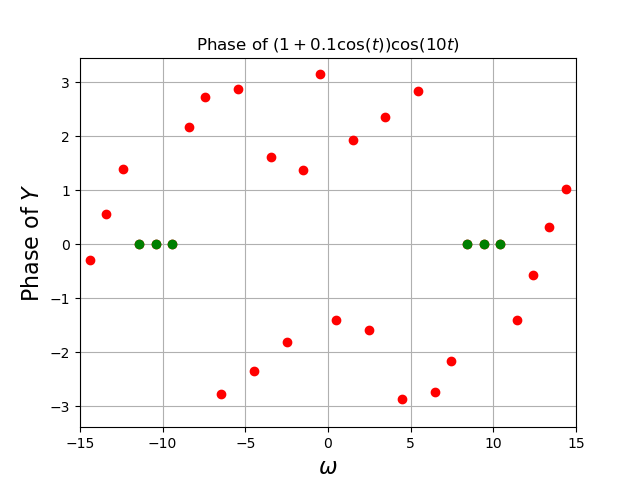
\includegraphics[scale = 0.75]{Figure_2b.png}
    \caption{Phase of (1 + 0.1cos(t))cos(10t) - 128 samples}
\end{figure}



\subsection{With only 512 Samples}
Plots:
\begin{figure}[H]
    \centering
    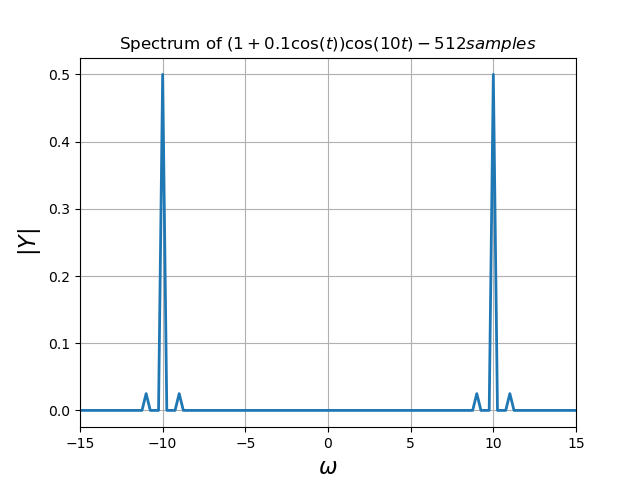
\includegraphics[scale = 0.75]{Figure_3a.png}
    \caption{Spectrum of (1 + 0.1cos(t))cos(10t) - 512 samples}
\end{figure}
\begin{figure}[H]
    \centering
    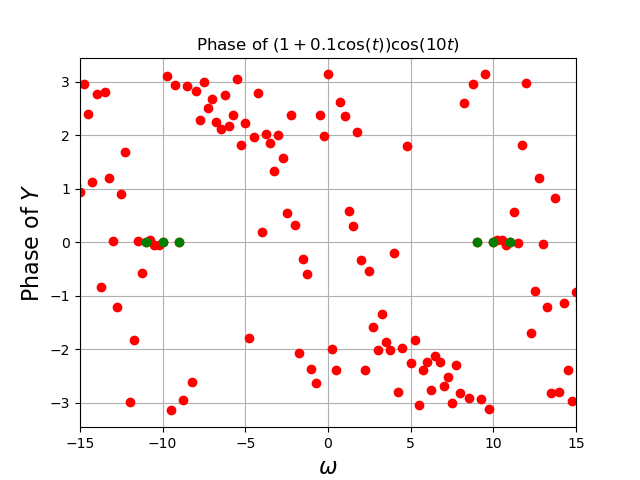
\includegraphics[scale = 0.75]{Figure_3b.png}
    \caption{Phase of (1 + 0.1cos(t))cos(10t) - 512 samples}
\end{figure}
We can clearly see that 6 peaks are not visible when we take a lower number of samples (i.e 128) but we the 6 peaks are clearly visible when we take a higher number of samples (i.e 512).\\~\\
Therefore, as we take more number of samples, a more accurate spectrum is achieved.

\subsection{Code}
\begin{python}
#DFT of (1 + 0.1cos(t))cos(10t) with 128 samples
t=linspace(0,2*pi,129);t=t[:-1]
y=(1+0.1*cos(t))*cos(10*t)
Y=fftshift(fft(y))/128.0
w=linspace(-64,63,129);w=w[:-1]

#Magnitude plot of the DFT of (1 + 0.1cos(t))cos(10t) with 128 samples
plot(w,abs(Y),lw=2)
xlim([-15,15])
ylabel(r"$|Y|$",size=16)
xlabel(r"$\omega$",size=16)
title(r"Spectrum of $\left(1+0.1\cos\left(t\right)\right)\cos\left(10t\right) - 128 samples$")
grid(True)
show()

#Phase plot of the DFT of (1 + 0.1cos(t))cos(10t) with 128 samples
plot(w,angle(Y),'ro',lw=2)
ii=where(abs(Y)>1e-3)
plot(w[ii],angle(Y[ii]),'go',lw=2)
xlim([-15,15])
ylabel(r"Phase of $Y$",size=16)
xlabel(r"$\omega$",size=16)
title(r"Phase of $\left(1+0.1\cos\left(t\right)\right)\cos\left(10t\right)$")
grid(True)
show()

#DFT of (1 + 0.1cos(t))cos(10t) with 512 samples
t=linspace(-4*pi,4*pi,513);t=t[:-1]
y=(1+0.1*cos(t))*cos(10*t)
Y=fftshift(fft(y))/512.0
w=linspace(-64,64,513);w=w[:-1]

#Magnitude plot of the DFT of (1 + 0.1cos(t))cos(10t) with 512 samples
plot(w,abs(Y),lw=2)
xlim([-15,15])
ylabel(r"$|Y|$",size=16)
xlabel(r"$\omega$",size=16)
title(r"Spectrum of $\left(1+0.1\cos\left(t\right)\right)\cos\left(10t\right)-512 samples$")
grid(True)
show()

#Phase plot of the DFT of (1 + 0.1cos(t))cos(10t) with 512 samples
plot(w,angle(Y),'ro',lw=2)
ii=where(abs(Y)>1e-3)
plot(w[ii],angle(Y[ii]),'go',lw=2)
xlim([-15,15])
ylabel(r"Phase of $Y$",size=16)
xlabel(r"$\omega$",size=16)
title(r"Phase of $\left(1+0.1\cos\left(t\right)\right)\cos\left(10t\right)$")
grid(True)
show()
\end{python}


\section{Spectrum of $sin^3t$ and $cos^3t$}
To compare the DFT of $sin^3t$ and $cos^3t$, we use the following:
\begin{equation}
    sin^3t = \frac{3sin(t)}{4} - \frac{sin(3t)}{4}
\end{equation}
\begin{equation}
    cos^3t = \frac{3cos(t)}{4} - \frac{cos(3t)}{4}
\end{equation}
Hence we observe the following:\\~\\
for $sin^3t$:
\begin{itemize}
    \item peaks at : w= 1 and -1, have a magnitude of 0.75
    \item peaks at : w= 3 and -3, have a magnitude of 0.25
    \item phase at w = -1,3 is $\frac{\pi}{2}$
    \item phase at w = 1,-3 is $-\frac{\pi}{2}$
\end{itemize}
Similarly for for $cos^3t$:
\begin{itemize}
    \item peaks at : w= 1 and -1, have a magnitude of 0.75
    \item peaks at : w= 3 and -3, have a magnitude of 0.25
    \phase of all the peaks will be 0.
\end{itemize}

\subsection{Plots of $sin^3t$}
\begin{figure}[H]
    \centering
    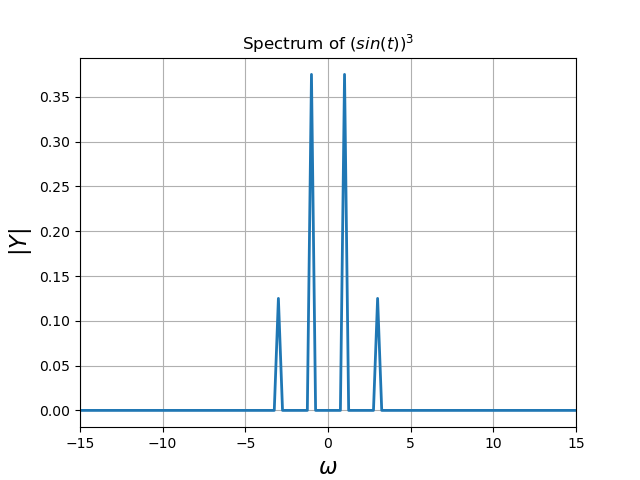
\includegraphics[scale = 0.75]{Figure_4a.png}
    \caption{Spectrum of sin^3t}
\end{figure}
\begin{figure}[H]
    \centering
    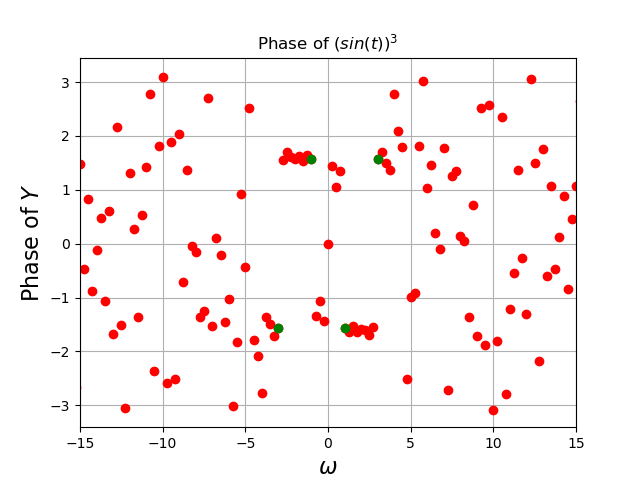
\includegraphics[scale = 0.75]{Figure_4b.png}
    \caption{Phase of sin^3t}
\end{figure}

\subsection{Plots of $cos^3t$}
\begin{figure}[H]
    \centering
    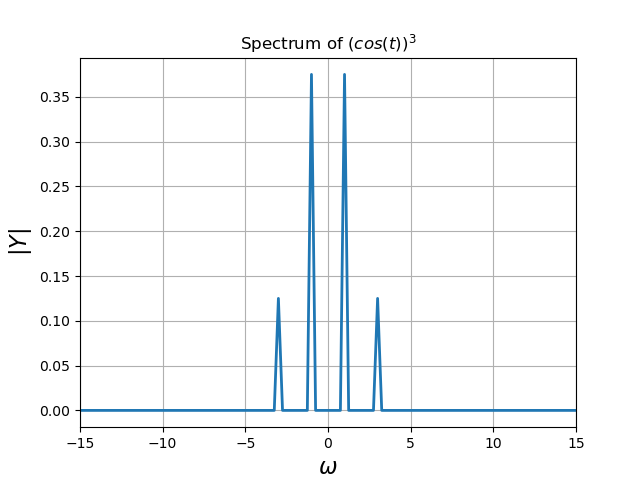
\includegraphics[scale = 0.75]{Figure_5a.png}
    \caption{Spectrum of cos^3t}
\end{figure}
\begin{figure}[H]
    \centering
    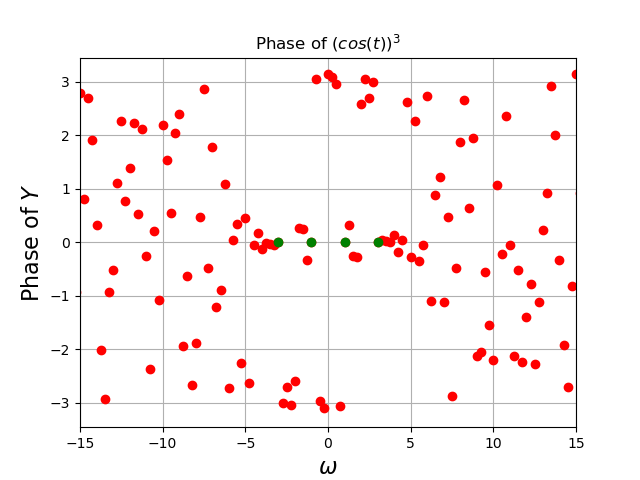
\includegraphics[scale = 0.75]{Figure_5b.png}
    \caption{Phase of cos^3t}
\end{figure}

\subsection{Code}
\begin{python}
#Q2: spectrums of (sin(t))^3 and (cos(t))^3

#DFT of (sin(t))^3 with 512 samples
t=linspace(-4*pi,4*pi,513);t=t[:-1]
y=(sin(t))**3
Y=fftshift(fft(y))/512.0
w=linspace(-64,64,513);w=w[:-1]

#Magnitude plot of the DFT of (sin(t))^3
plot(w,abs(Y),lw=2)
xlim([-15,15])
ylabel(r"$|Y|$",size=16)
xlabel(r"$\omega$",size=16)
title(r"Spectrum of $(sin(t))^3$")
grid(True)
show()

#Phase plot of the DFT of (sin(t))^3
plot(w,angle(Y),'ro',lw=2)
ii=where(abs(Y)>1e-3)
plot(w[ii],angle(Y[ii]),'go',lw=2)
xlim([-15,15])
ylabel(r"Phase of $Y$",size=16)
xlabel(r"$\omega$",size=16)
title(r"Phase of $(sin(t))^3$")
grid(True)
show()



#DFT of (cos(t))^3 with 512 samples
t=linspace(-4*pi,4*pi,513);t=t[:-1]
y=(cos(t))**3
Y=fftshift(fft(y))/512.0
w=linspace(-64,64,513);w=w[:-1]

#Magnitude plot of the DFT of (cos(t))^3
plot(w,abs(Y),lw=2)
xlim([-15,15])
ylabel(r"$|Y|$",size=16)
xlabel(r"$\omega$",size=16)
title(r"Spectrum of $(cos(t))^3$")
grid(True)
show()

#Phase plot of the DFT of (cos(t))^3
plot(w,angle(Y),'ro',lw=2)
ii=where(abs(Y)>1e-3)
plot(w[ii],angle(Y[ii]),'go',lw=2)
xlim([-15,15])
ylabel(r"Phase of $Y$",size=16)
xlabel(r"$\omega$",size=16)
title(r"Phase of $(cos(t))^3$")
grid(True)
show()
\end{python}



\section{Spectrum of Phase Modulated signal cos(20t +5cos(t))}
\subsection{Plots}

\subsection{Plots of cos(20t +5cos(t))}
\begin{figure}[H]
    \centering
    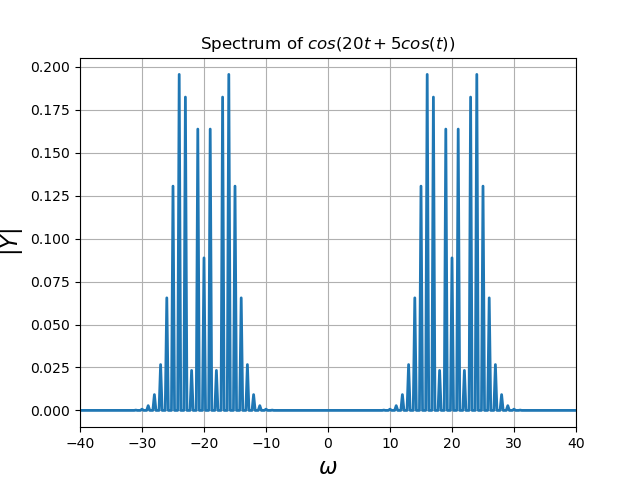
\includegraphics[scale = 0.75]{Figure_6a.png}
    \caption{Spectrum of cos(20t +5cos(t))}
\end{figure}
\begin{figure}[H]
    \centering
    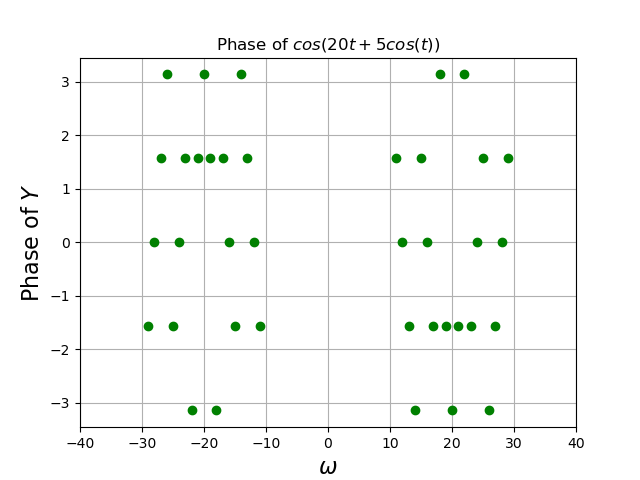
\includegraphics[scale = 0.75]{Figure_6b.png}
    \caption{Phase of cos(20t +5cos(t))}
\end{figure}

\subsection{Analysis}
\begin{itemize}
    \item We have plotted the spectrum of cos(20t +5cos(t)) for a time interval of $(-4\pi,4\pi)$ and for 512 number of samples.
    \item We have only plotted the phase for points with a magnitude greater than $1e^{-3}$.
    \item We can clearly see that in the phase plot of the signal, all the points are centered around the carrier frequency of w=20
    \item Hence, its clear that the signal is a Phase Modulated signal.
\end{itemize}

\subsection{Code}
\begin{python}

#Q3: spectrum of phase modulated signal cos(20t +5cos(t))

#DFT of cos(20t +5cos(t)) with 512 samples
t=linspace(-4*pi,4*pi,513);t=t[:-1]
y=cos(20*t+5*cos(t))
Y=fftshift(fft(y))/512.0
w=linspace(-64,64,513);w=w[:-1]

#Magnitude plot of the DFT of cos(20t +5cos(t))
plot(w,abs(Y),lw=2)
xlim([-40,40])
ylabel(r"$|Y|$",size=16)
xlabel(r"$\omega$",size=16)
title(r"Spectrum of $cos(20t +5cos(t))$")
grid(True)
show()

#Phase plot of the DFT of cos(20t +5cos(t))
ii=where(abs(Y)>1e-3)
plot(w[ii],angle(Y[ii]),'go',lw=2)
xlim([-40,40])
ylabel(r"Phase of $Y$",size=16)
xlabel(r"$\omega$",size=16)
title(r"Phase of $cos(20t +5cos(t))$")
grid(True)
show()
\end{python}


\section{Spectrum and Analysis of the Gaussian function}
A Gaussian Function is a function of the form:
\begin{equation}
    f(x) = ae^{-\frac{(x-b)^2}{2c^2}}
\end{equation}
In our case, the function is:
\begin{equation}
    f(t) = e^{-\frac{t^2}{2}}
\end{equation}
This function is very useful as its fourier transform is also a gaussian function.\\~\\
The fourier transform of the given signal is:
\begin{equation}
    Y(w) = \frac{1}{\sqrt{2\pi}}e^{-\frac{w^2}{2}}
\end{equation}
\begin{itemize}
    \item Its important to remember that the given signal is \textbf{aperiodic}, hence it is not bandlimited in the frequency domain.
    \item Hence, the spectrum depends on the time interval and the number of samples we take.
    \item since the signal is real, the phase plot will be completely 0. Hence we dont have to plot it. 
\end{itemize}
To plot the spectrum, we consider 2 different number of samples and time intervals,
\begin{itemize}
    \item N=1024, $-16\pi,16\pi$
    \item N=512, $-8\pi,8\pi$
\end{itemize}


\subsection{For $-16\pi,16\pi$ and 1024 samples}
\begin{figure}[H]
    \centering
    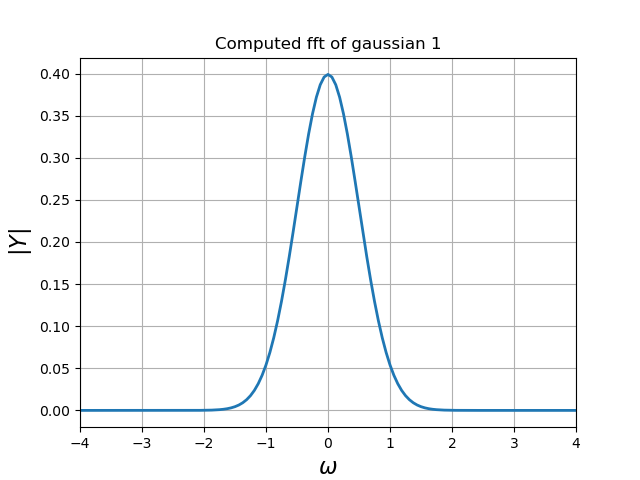
\includegraphics[scale = 0.75]{Figure_7a.png}
    \caption{Spectrum of gaussian function}
\end{figure}

\subsection{For $-8\pi,8\pi$ and 512 samples}
\begin{figure}[H]
    \centering
    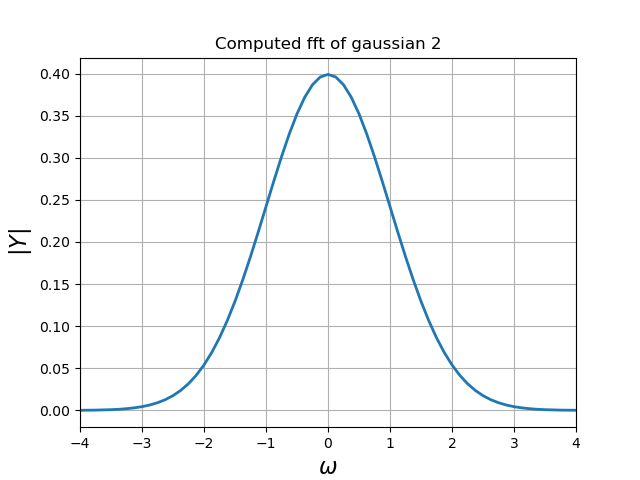
\includegraphics[scale = 0.75]{Figure_7b.png}
    \caption{Spectrum of gaussian function}
\end{figure}

Hence, we can see that the spectrum of the gaussian sharpens as we increase the number of samples taken and reduce the time interval (i.e, we increase the sampling rate).\\~\\
We plot the actual gaussian function and see that it strongly coincides with the Figure 14. (i.e $-8\pi,8\pi$ range and 512 samples) with minimal deviation.\\~\\
We cross check this by finding the maximum deviation, which is equal to \textbf{$1.608160*10^{-16}$} which is extremely small.

\subsection{Actual Gaussian function plot}
\begin{figure}[H]
    \centering
    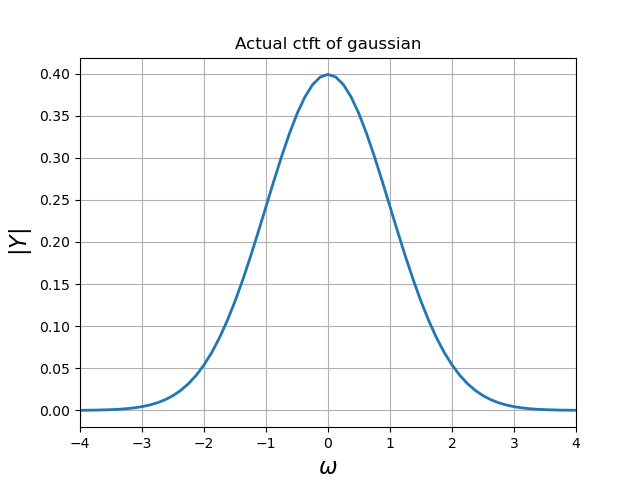
\includegraphics[scale = 0.75]{Figure_7c.png}
    \caption{Spectrum of actual gaussian function}
\end{figure}

\subsection{Code}
\begin{python}
#Q4: spectrum of Gaussian Function with different sampling rates

#case1 : sampling rate is higher
T=16*pi
N=1024
N2=512

#spectrum of the gaussian function
t = linspace(-T/2,T/2,N+1);t=t[:-1]
y = exp(-(t**2)/2)
Y = fftshift(abs(fft(y)))/N # Finding DFT
Y = Y/(max(Y)*sqrt(2*pi))
w = linspace(-N2*pi/T,N2*pi/T,N+1);w=w[:-1]
fft_gf = (1/sqrt(2*pi))*exp(-(w**2)/2)

#plotting the spectrum
plot(w,abs(Y),lw=2)
xlim(-4,4)
title('Computed fft of gaussian 1')
ylabel(r"$|Y|$",size=16)
xlabel(r"$\omega$",size=16)
grid(True)
show()


#case2 : sampling rate is lower
T=16*pi
N=512
N2=512

#spectrum of the gaussian function along with the ctft of the ACTUAL gaussian function
t = linspace(-T/2,T/2,N+1);t=t[:-1]
y = exp(-(t**2)/2)
Y = fftshift(abs(fft(y)))/N # Finding DFT
Y = Y/(max(Y)*sqrt(2*pi))
w = linspace(-N2*pi/T,N2*pi/T,N+1);w=w[:-1]
fft_gf = (1/sqrt(2*pi))*exp(-(w**2)/2)
error = max(abs(abs(Y)-fft_gf)) #finds the maximum error between the calculated and actual functions

#plotting the spectrum
plot(w,abs(Y),lw=2)
xlim(-4,4)
title('Computed fft of gaussian 2')
ylabel(r"$|Y|$",size=16)
xlabel(r"$\omega$",size=16)
grid(True)
show()

#plotting the spectrum of the ACTUAL gaussian function
plot(w,abs(fft_gf),lw=2)
xlim(-4,4)
title('Actual ctft of gaussian')
ylabel(r"$|Y|$",size=16)
xlabel(r"$\omega$",size=16)
grid(True)
show()

print('The Maximum error between the computed and actual fft of the gaussian function is %e:' %error)
\end{python}

\section{Conclusion}
\begin{itemize}
    \item In this assignment, we have learnt how to find the DFT of various signals with the help of the fft numpy module (fft and fftshift).
    \item We analysed the data and plotted the respective spectrum and phase plot.
    \item We analysed the DFT for: 
    \begin{enumerate}
        \item Sinusoids
        \item Amplitude modulated signals
        \item Phase modulated signals and
        \item The Gaussian function
    \end{enumerate}
    \item We have seen how for the phase modulated signal, the phase plot is centered around w=20 and is zero for most values far away from it.
    \item We have seen how the gaussian function has multiple spectrums based on the time interval and the samples taken,
    \begin{enumerate}
        \item The Plot sharpens as we decrease the time interval and
        \item The plot sharpens as we decrease the number of samples, i.e
        \item the plot sharpens for a higher sampling rate.
    \end{enumerate}
\end{itemize}















\end{document}

